\chapter{Enabling Temporal Neural Networks via Geometric Tensor Representations} \label{chap:ott} 

While feature selection dates back to classical statistics, 
\textit{parameter selection} has only recently been
studied as
the dimensionality and complexity of models grows
linearly with the size of modern neural networks.
Recurrent Neural networks (RNNs) and its variants are the de facto 
tool of choice 
for modeling sequential data in machine learning and vision.
%For high-dimensional data, a large problem initially faced by these models included exploding/vanishing gradients. 
But until only recently, these models have been severely limited in their ability to model high-dimensional data.
Recurrent structures often lead to large model sizes dependent on sequence length, and thus also require an equivalent number of increased computation.
While RNNs have been successfully applied to video data in some cases, the strategy 
requires problem specific innovations because of the large mapping necessary 
from inputs to hidden representations. It is fair to say that the growth 
in the number of model parameters in various types of 
recurrent models remains a serious bottleneck for high 
dimensional datasets. 
%
% Convolutional neural networks (CNNs), on the other hand, 
% %better suited at 
% handle high dimensional data
% %Modern deep learning architectures now almost exclusively use Convolutional neural networks (CNNs) %to alleviate this issue. 
% %CNNs, partly due to how most networks in broad use today are set up,
% far better and 
% can reduce the dimension of an input significantly by deriving rich feature maps. Most computer vision tasks involve some form of a CNN within the architecture, but incorporating CNNs within recurrent structures 
% seamlessly to mitigate the RNN specific model size issues described above is not always straightforward. Notice that a direct replacement of input and output layers with CNNs leads to a shrinkage of the sequence length considerably \cite{srivastava2015unsupervised}, and pre-training CNN layers may lead to poor local minima when we train without using an end-to-end pipeline \cite{donahue2015long}. Some recent works suggest the use of dilated convolutional networks 
% for sequence modeling \cite{yu2015multi} to partly mitigate these issues, but this line of work is still in its early stages. 
%A similar issue exists with other 
For model-size reduction, both for RNN style networks and otherwise, 
PCA or random projections \citep{ye2005two,bingham2001random} style ``compression" ideas have 
also been used with varying degrees of success.

An interesting perspective on the effective degrees of freedom afforded 
by a given network, a surrogate for the actual ``size'' of the architecture, 
is provided by tensor methods.
% and traces its roots to early 
%results in approximation theory and numerical linear algebra. 
%distinct but related line of work is on t
Tensor decomposition based methods have recently been shown to enable low dimensional representations of very high dimensional data, 
and while these ideas were known to be effective in the ``shallow" regime much earlier, new results also demonstrate their applicability for deep neural 
networks. 
In particular, in the last year, we see a number of tensor based methods being successfully adapted for deep neural network design and compression \citep{cohen2016expressive,zhang2017tucker,yu2017compressing}.
Specifically, \citep{pmlr-v70-yang17e} shows that these compression methods can be very effective in reducing the parameter cost of weight layers in RNNs, enabling simple video analysis tasks that previously would have been computationally prohibitive.

Our goal is to design rich sequential or recurrent models to analyze a longitudinal sequence of high dimensional 3D brain images. 
This task raises two major issues. \textbf{First}, 
unless the model size is parsimonious, we find that merely instantiating the 
model with data involving 3D images over multiple time points, even on multiple high end GPU instances, is challenging.
\textbf{Second}, 
the eventual goal of medical image analysis is either scientific discovery or generating 
actionable knowledge for patient betterment. 
Both goals require evaluating a model's confidence via 
classical or contemporary statistical techniques: for instance, how confident is the model of its prediction?  
Most, if not all, available tools for assessing 
model uncertainty of deep neural network models 
have a strong dependence on the number of parameters in 
the model. Therefore, even if the first issue above could be mitigated by clever implementation ideas, purely as a practical 
matter, the design of rich and expressive models with a small number of parameters yields immense benefits for calculating model uncertainty.

\textbf{The Central Idea.}
Let $\cX \in \RR^{n_1 \times \cdots \times n_d}$ be a $d$-dimensional array, or tensor, with each mode having length $n_i$. To store a full rank tensor, $n^d$ storage would be required. A number of tensor factorizations have been developed to reduce this storage cost. The CANDECOMP/PARAFAC (CP) \citep{harshman1970foundations,carroll1970analysis} decomposition reduces the storage to $O(dnr)$, but finding the exact CP-rank $r$ is NP-hard. Hierarchical tensor methods have also proven to be effective in tensor compression \citep{cohen2016expressive, cohen2016convolutional}.

The \textit{Tensor Train} decomposition (TT) \citep{oseledets2011tensor}, defines an element of the tensor as
\begin{align}
\cX(x_1,\ldots,x_d) = A_1(x_1)\cdots A_d(x_d)
\end{align}
where $x_i \in \left\{1,\ldots, n_i\right\}$, and $A_i(x_i) \in \RR^{r_{i-1} \times r_{i}}$ for each $i \in \{1,\ldots,d\}$ are called the \textit{cores} of the tensor train, with $r_0 = r_d = 1$. Equivalently, the full tensor is written as:
\begin{align}\label{eq:fullTT}
\cX &= \sum_{k_0 = 1}^{r_0} \cdots \sum_{k_d = 1}^{r_d} A_1(k_0,:,k_1) \otimes \cdots \otimes A_d(k_{d-1},:,k_d) 
\end{align}
where $A_i \in \RR^{r_{i-1}\times n_i \times r_i} $. This format requires $O(dnr^2)$ storage, but has two major advantages over the CP format. First, finding the TT-rank (the smallest set of $r_i$'s that satisfy the decomposition with equality) of any arbitrary tensor is tractable, and as such all tensors can be efficiently rewritten in the TT format. Second, projecting arbitrary tensors onto the TT format of a fixed rank requires only a set of QR and singular value decompositions \citep{oseledets2011tensor}. This projection, \textit{TT-rounding}, additionally allows for a given TT tensor of some rank to be projected onto the space of TTs with lower rank, and requires $O(dr^3)$ computational complexity. Separately, specific tensor train constructions have recently been identified as forms of general recurrent networks \citep{khrulkov2018generalized}

Ideally, we would prefer a construction which keeps the standard TT-core format and involves optimization over ``smaller'' Stiefel manifolds. Consider the following representation, in which each TT-core itself is orthogonal.
\begin{definition}\label{def:ott}(Orthogonal Tensor Train)
	The Orthogonal Tensor Train is defined as
	\begin{align}
	\cX(x_1,\ldots,x_d) = Q_1(x_1) \cdots Q_d(x_d),
	\end{align}
	where each $Q_i(x_i)$ lies on the Stiefel $\ST(m_i, M_i)$, where $m_i = \min(r_{i-1},r_i)$, and  $\ M_i = \max(r_{i-1},r_i)$.
\end{definition}
While in this formulation the total number of components in the product space of Stiefels is $nd$, the dimension of each manifold is {\bf significantly smaller},
dependent {\em only} on the core rank as opposed to the mode size.
The total number of parameters, if $n_i =n, r_i = r$, is
\begin{align}
n \sum_{i=1}^d \left[ r^2 - \frac{r^2 + r}{2}\right] = d n r^2 - dn\frac{r^2 + r}{2}.
\end{align}
When compared to the full TT representation,
the Orthogonal Tensor Decomposition (OTT) requires
$(r+1)/2r \approx 1/2$ as many parameters.
If $r_i=r_{i+1}$, then $\ST(m_i, M_i) = SO(m_i)$, where $SO$ is the special orthogonal group.

This construction can be seen as an approximation to the full tensor train format, in which the upper triangular part of each core is set to identity:
\begin{align*}
&\cX(x_1,\ldots,x_d) = A_1(x_1)\cdots A_d(x_d) \\ &= Q_1(x_1)R_1(x_1)\cdots Q_d(x_d)R_d(X_d) \\
&\approx Q_1(x_1) \cdots Q_d(x_d) %\numberthis
%&= \sum_{r_0}\cdots\sum_{r_d} A_1(x_1)[r_0,r_1]\cdots A_d(x_d)[r_{d-1},r_d].
\end{align*}

\begin{algorithm}[H]
	\begin{algorithmic}
		\For{t=1,\ldots,T}
		\State $g_t := \frac{df}{d\cW} f(X^{mini-batch})$
		\For{Core $Q^i_t \in \cW_t$ and Core Gradient $g^i_t \in g_t$}
		\State $G^i_t = P_{T_{\cW_t}M}(g^i_t)$ \Comment{Projection Step}
		\State $Q^i_{t+1} \leftarrow \Exp(Q^i_t, G^i_t)$ \Comment{Retraction Step}
		\EndFor
		\EndFor
	\end{algorithmic}
	\caption*{\footnotesize Stochastic OTT Optimization}
\end{algorithm}

\begin{figure}
	\centering
	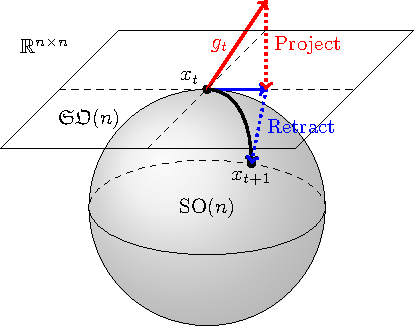
\includegraphics[width=0.5\columnwidth,trim={0 1.5cm 0 0},clip]{chap3/stiefel_update.pdf}
	\caption{\footnotesize Visualization of the gradient descent update using the projection and retraction on the Stiefel manifold. The update is applied to each core individually, allowing for smaller manifold operations that would otherwise scale poorly with dimension.}
\end{figure}


%\begin{figure*}[ht]
%	%	\captionsetup[subfigure]{labelformat=empty}
%	%	\centering
%	\begin{subfigure}{.49\textwidth}
%		\centering
%		\begin{algorithm}[H]
%			\begin{algorithmic}
%				\For{t=1,\ldots,T}
%				\State $g_t := \frac{df}{d\cW} f(X^{mini-batch})$
%				\For{Core $Q^i_t \in \cW_t$ and Core Gradient $g^i_t \in g_t$}
%				\State $G^i_t = P_{T_{\cW_t}M}(g^i_t)$ \Comment{Projection Step}
%				\State $Q^i_{t+1} \leftarrow \Exp(Q^i_t, G^i_t)$ \Comment{Retraction Step}
%				\EndFor
%				\EndFor
%			\end{algorithmic}
%			\caption*{\footnotesize Stochastic OTT Optimization}
%		\end{algorithm}
%		\caption{\label{alg:ott_opt}}
%	\end{subfigure}%
%	\hfill
%	\begin{subfigure}{.49\textwidth}
%		\centering
%		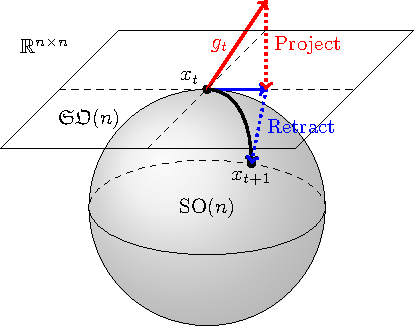
\includegraphics[width=0.85\columnwidth,trim={0 1.5cm 0 0},clip]{chap3/stiefel_update.pdf}
%		\caption{}
%	\end{subfigure}
%	\vspace{-10pt}
%	\captionof{figure}{\label{fig:ott_opt}\footnotesize Algorithm (a) and visualization (b) of the gradient descent update using the projection and retraction on the Stiefel manifold. The update is applied to each core individually, allowing for smaller manifold operations that would otherwise scale poorly with dimension.}
%\end{figure*}

\textbf{Goals.} Using this construction, we will tackle the problem of modeling 
sequential 3D brain imaging data using 
recurrent/sequential models. 
Our development starts from well known results on tensor decomposition, and in particular, we
make use of the tensor train representation, which has been shown to be effective in several 
applications in vision and machine learning. We derive a reformulation of the decomposition using 
orthogonality constraints and show that while this makes the estimation slightly more challenging, 
it reduces the number of parameters by as much as half. 
We present a novel parameter estimation scheme based on Stiefel manifold optimization and demonstrate 
how the end to end construction yields benefits for convergence and uncertainty estimation. 
Finally, from the empirical side, we will discuss how we enable analysis of and prediction using sequential 3D brain imaging datasets, which to our knowledge is the first such result using 
deep recurrent/sequential architectures. 
